\section{Introduction}
Imagine that six months ago your team decided to adopt \quotes{Collective Code Ownership.} You have enjoyed the freedom to be able to change any part of the code base. You remember that as you were implementing a feature, you found an unreported bug and simply fixed it. In fact, fixing it was easier than creating a ticket and asking the former owner to change it. Just last week, you refactored a pattern that spanned the entire system without needing to coordinate a team meeting in order to get everyone on the same page. Yet, something does not feel quite right: you literally shuddered when you looked at the Service Manager for all of its complexity and obtuse code. The creator of the Service Manager was smart, maybe too smart, but not smart enough to simplify the design. Unfortunately, the creator left the company a few months back.  While your team is permitted to modify every part of the code, you realize that you are unable to do so. Worse yet, is the underlying feeling that your team doesn't have the ability to change certain parts of the system and so cannot \quotes{own} all the code.

Shifting from individual to collective code ownership is not simple; it requires multiple and complementary practices which enable a team to actively remove knowledge silos. For example, instead of strong code ownership where one developer implements a complex feature, many developers can now shape its implementation as the baton of development is rotated through the team. 

%The theory of sustainable software development through collective code ownership \cite{SustainableSoftwareDevelopment} introduced a solution to the problem of handling disruptions such as vacations, rotation of team members, churn, and growing team size. The theory fosters cross-sharing knowledge and simplifying code to make it easy to maintain. The theory is composed of six synergistic practices: Pair Programming, Overlapping Pair Rotation, Knowledge Pollination, Test Driven Development / Behavior Driven Development, Continuous Refactoring, and Live on Master. These practices work when the business adopts three policies: Shared Schedule, Avoid Technical Debt, and Collective Code Ownership.

%The sustainable software development theory requires a shift from individual code ownership to collective code ownership. Instead of strong code ownership, where one developer implements a complex feature, many developers shape the implementation of a feature as the baton of development is rotated through the team. 


This paper emerged from an iterative research method called Grounded Theory. We collected empirical data from participant observations of an Extreme Programming project at Pivotal and through interviews of Pivotal engineers, designers, and product managers. %As aspects of the theory emerged, we collected additional data to validate and saturate the theory.

Our initial core question was: \quotes{What is happening at Pivotal when it comes to software development?} When \quotes{collective code ownership} emerged as a core category, we collected additional sampling to identify which situations which would impact a programmer's sense of ownership and to identify which practices were required to enable collective code ownership. 

In this paper, we examine which dimensions, or factors, affect the team's sense of ownership.

In section \ref{RelatedWork}, we position the research relative to existing literature regarding collective code ownership. In section \ref{ResearchMethod}, we review how we employed Grounded Theory to derive a theory supported by empirical data. In section \ref{ResearchContext}, we present the research context by explaining Pivotal's background. In section \ref{CollectiveCodeOwnership}, we examine the benefits and potential threats to collective code ownership. In section \ref{Transitioning}, we examine nuanced issues of transitioning to collective code ownership. In section \ref{TheoryEvaluation}, we evaluate the theory using established criteria for evaluating a grounded theory. In the last sections, we examine threats to research validity, future research, and conclude the research.



\section{Related Work}
\label{RelatedWork}
In Extreme Programming (First Edition) \cite{ExtremeProgramming2000} Kent Beck describes a set of interdependent practices that manage feature development (much like Scrum \cite{Scrum}), as well as technical practices that facilitate a collaborative team environment. Both of these elements are essential to create a team which routinely delivers value to its customers.

Kent Beck succinctly discusses the Collective Ownership practice: he contrasts Collective Ownership against \quotes{no ownership} and \quotes{individual ownership.} He summarizes, \quotes{In XP, everybody takes responsibility for the whole of the system. Not everyone knows every part equally well, although everyone knows something about every part. If a pair is working and they see an opportunity to improve the code, they go ahead and improve it if it makes their life easier.}  \cite{ExtremeProgramming2000}

In Extreme Programming (Second Edition) \cite{ExtremeProgramming2004}, Kent Beck refines Extreme Programming into 13 primary practices and 11 corollary practices. He renames Collective Ownership to Shared Code and distills the practice into: \quotes{Anyone on the team can improve any part of the system at any time.} 

In 2006, Martin Fowler defined collective code ownership, similarly to Beck \cite{FowlerCodeOwnership}, as a contrasting team position to \quotes{strong code ownership}. In strong code ownership, each file is owned by one person and \quotes{weak code ownership} where developers can change files, but an owner keeps an eye on files for which they are responsible. 

In 2011, Christian Bird et al \cite{BirdDontTouchMyCode} contrasted the effects of strong- and weak-ownership. The demonstrated that weak ownership lead to more defects than strong ownership for Windows Vista and Windows 7. The study defined ownership for a software component as a percentage of the version control commits for a single developer. They defined a major contributor as someone who has more than 5\% of the git commits. A sensitivity analysis revealed that defining strong code ownership as a range from 2\% to 10\% produced similar results for the study.

In 2015, Brendan Murphy stated that the concept of code ownership must been unpacked and expanded. He argued: the complexities of code ownership are missed by merely examining git commits to determine who modified which files. \cite{MurphyIEEESoftware}.

Collective code ownership requires more than a team saying, \quotes{everyone can modify anything.} Instead, this paper is interested in how much the team feels that they collectively own the code. We define \quotes{sense of collective code ownership} as the degree to which individual members of the team feel collective ownership.  

\section{Research Method: Grounded Theory}
\label{ResearchMethod}

We followed Charmaz' approach to Grounded Theory \cite{Charmaz} which provides an iterative approach to data collection, data coding, and analysis resulting in an emergent theory. The two primary data sources were field notes collected during continuous participant observations of a 7.5 month project and interviews with Pivotal software engineers, designers, and product managers. Interviews were recorded, transcribed, coded, and analyzed using constant comparison. 

%Grounded Theory immerses the researcher within the context of the research subject from the point of view of the participants. As the research progresses, Grounded Theory allows the researcher to \quotes{incrementally direct the data collection and theoretical ideas.} The theory provides a starting place for inquiry, not a specific goal known at the beginning of the research. As we interact with the data, the data influences how we progress and alters the research direction. 
When starting a grounded theory research study, the core question is \quotes{What is happening here?}' (Glaser, 1978) \cite{GlaserTheoreticalSensitivity}. Our initial core question was: \quotes{What is happening at Pivotal when it comes to software development?}

\subsection{Participants}
The primary researcher interviewed 21 engineers, product managers, and designers who had experience with Pivotal's software development process. Participants were not paid for their time. 
\subsection{Interviewing}
The primary researcher relied on \quotes{intensive interviews} which Charmaz summarizes as \quotes{open-ended yet directed, shaped yet emergent, and paced yet unrestricted} \cite{Charmaz}. The technique relies on open-ended questions. The purpose is for the researcher to enter into the participant's personal perspective within the context of the research question. %The interviewer needs to abandon assumptions and their own personal presumptions in order to understand and explore the interviewee's perspective. %Charmaz \cite{Charmaz} contrasts intensive interviews from informational interviews which endeavor to collect accurate `facts' and investigative interviews that attempt to reveal hidden intentions or expose practices and policies. 
 
%The interviews were open-ended explorations starting with the question, ``please draw on this sheet of paper, your view of Pivotal's software development process." The interviewer specifically didn't force initial topics and merely followed the path of the interviewee. 

After the first round of interviews, analytical work revealed emergent categories which were then explored deeper in subsequent interviews. While exploring new emergent core categories, whenever possible, the researcher initiated subsequent interviews with a goal of not forcing the issue. For example, ``please draw your feelings about the code" often resulted in conversations about code ownership. 

After the interview, the interview was transcribed into a Word document with timecode stamps for each segment.

\subsection{Field Notes}
In addition to collecting data from interviews, the primary researcher collected field notes while working as a engineer. The field notes comprise of multiple paragraph entries recorded several times a week collected over a six month period. The field notes describe individual and collective actions, captures what participants defined as interesting or problematic, and include anecdotes and observations. 
\subsection{Initial Coding}
The primary researcher followed line-by-line coding as recommended by Charmaz \cite{Charmaz}. The line-by-line coding helps the researcher slow down and examine for nuanced interactions in the data. Based upon Charmaz's advice, the primary researcher adopted a coding scheme that was simple, direct, analytic, and spontaneous.  

After the initial coding, another researcher reviewed the initial codes while reading the transcripts and listening to the audio recording. During a weekly research collaboration meeting, any concerns were discussed and addressed. During these meetings, we recorded and transcribed into grounded theory memos any discussions about analysis or understanding the codes. Recording the sessions mitigated Glazer's concerns about missing possible memos or insights that are verbally discussed. \cite{GlaserTheoreticalSensitivity}

Once emergent themes arrive, then coding in later parts of the research were focused around the themes. The focused coding phase allowed the primary researcher to ``sort, synthesize, integrate, and organize large amounts of data."
\subsection{Constant Comparison, Focused Coding, and Memoing}
As data was collected and coded, the researcher placed codes into a spreadsheet organized based on focused codes. Only ideas shared by multiple interviewees earned their way into focused codes and subsequent analysis. The researcher compared new codes to existing codes for emergence of new categories. The primary researcher periodically audited each category by comparing the codes to each other and verifying the cohesion of the category. For complex categories, the codes were printed onto index cards, arranged and re-arranged until the emergence of logical categories.  The researcher captured the analysis of codes, examinations of theoretical plausibility, and insights in memos. 

\subsection{Theoretical Sampling}
As theoretical codes emerged, the researcher altered data collection for saturating core categories. When collective code ownership emerged as a core category, additional sampling was collected to identify which situations would increase or decrease a programmer's sense of ownership and which practices were required to enable collective code ownership.

\section{Research Context}
\label{ResearchContext}
\subsection{Organizational Context: Pivotal}
Pivotal provides solutions for cloud-based computing, big data, and agile development. Pivotal Cloud Foundry is an open source Platform as a Service either on-premise or hosted in the cloud. Pivotal Big Data Suite stores and analyzes multiple large data sets using Hadoop, Hawq, and Green Plum. Pivotal Labs provides agile developers and designers for startups and enterprise companies to transform their software development process. Pivotal Labs has 16 offices around the world.

Pivotal Lab's mission is to both deliver highly-crafted software products and provide a transformative experience for their client's engineering cultures. In order to change a developer's way of working, Pivotal combines the client's software engineers with Pivotal's engineers at a Pivotal office where they can experience Extreme Programming in an environment conducive for agile development. This experience is similar to the creation of the NUMMI plant where General Motors sent workers to Japan to learn Toyota's Production System \cite{Nummi}. For startups, Pivotal might be the first engineers working on the project. For enterprise clients, Pivotal provides additional engineering resources to accomplish new business goals. Sometimes, Pivotal helps transform engineering cultures when they no longer routinely deliver code.  

Common team sizes are six developers with a designer and a product manager. In the Palo Alto office, the number of developers on a project currently ranges from 2, 4, 6, 8, 10, 22, and 28. Larger projects are decomposed into smaller coordinating teams with one product manager per team and one or two designers per team. 

Commonly utilized technologies include Angular, Android, backbone, iOS, Java, Rails, React, and Spring often deployed onto Pivotal's Cloud Foundry. 

Pivotal Labs has followed Extreme Programming \cite{ExtremeProgramming2004} since the late 1990's. While each team is autonomous in making its own decisions as to what is best for a particular project, the company culture strongly suggests following all of the core practices of Extreme Programming including Pair Programming, Test Driven Development, Weekly Retrospectives, Daily Stand-ups, Prioritized Backlog, Whole Team ownership of the project and code base, plus Kanban's notion of work flowing through people.

% In addition to the lengthy intensive interviews, the primary researcher asked all of the software engineers, designers, and product managers at the Palo Alto office the question, \quotes{Given all of the values, principles, and practices of Pivotal, what do you think is the heart of the matter, what is core to all we do?} Table \ref{CorePractice} includes the various answers. The diversity of answers shows that there is no common understanding as to what is core. 

% \begin{table}[t]
% \renewcommand{\arraystretch}{1.3}
% \centering
% \caption{Asking \quotes{What is core to all we do?} shows that there is no clear understanding of fundamental}
% \label{CorePractice}
% \begin{tabular}{|p{3.10in}|}
% \hline
% empathy \\ \hline
% teamwork \\ \hline
% communication \\ \hline
% doing things the right way \\ \hline
% constant communication \\ \hline
% collaboration \\ \hline
% pairing, TDD \\ \hline
% TDD, agile planning, pair programming \\ \hline
% feedback, fast feedback loop \\ \hline
% kindness, no matter what you do, if you hurt people, that's not good. Software is built by humans. Act human \\ \hline
% user research and feedback \\ \hline
% delivery of value to the customer \\ \hline
% keeping clients paying us means that I have a job. Pairing has a very real impact in attracting clients. TDD has large impact on code quality. Once I leave pivotal, TDD is what I will take to my next job \\ \hline
% doing the right thing \\ \hline
% iteration practices drive our other practices. We do lean design. Build Measure Learn \\ \hline
% short feedback loops both at the project level and personal level when people giving me feedback \\ \hline
% empathy \\ \hline
% pairing, testing \\ \hline
% self reflection and  team retros \\ \hline
% doing the right thing \\ \hline
% enabling companies to build great software \\ \hline
% guaranteed repeatable success \\ \hline
% kindness, feedback loops, bias towards action \\
% \hline
% \end{tabular}
% \end{table}
\section{Collective Code Ownership}
\label{CollectiveCodeOwnership}

In the literature, collective code ownership is treated as a policy statement. In practice, a team claiming that \quotes{anyone can modify any piece the code} is not sufficient to achieve the desired results. 

The theory of sustainable software development presents a set of related practices that must be in place to achieve collective code ownership. 

The sense of collective code ownership is a spectrum. On one side, each individual has ownership of only their code;  on the other side, everyone on the team owns the entire code base. A team striving for collective code ownership may land somewhere in between. 

Our research revealed that the sense of collective code ownership is dynamic. Negative project influences can erode the team's sense of ownership over the project's duration. A team needs to counteract these erosions in order to increase their sense of ownership. Ownership is an emotional or qualitative attribute which ties all developers on the team to the project and code base..

% People, not machines, create software, and as such, we need to factor psychological considerations. As one engineer expressed, \quotes{We are people [and our interactions with the code is as meaningful as the code itself].} Listening, caring, and empathizing with one another allows the team to work through differences of opinion towards a stronger code base. One designer said, \quotes{You have to be an adult to work here.} Letting go of personal ownership enables the team to achieve collective code ownership. Sustainable Software Development fosters an environment where the whole is more than the sum of the parts. 

\subsection{Research Question 1: What fosters the developer's sense of collective code ownership?}
At Pivotal, developers learn in time to loosely hold personal contributions; they recognize the lack of long term individual authorship. Three practices contribute to this dynamic: Pair Programming, Overlapping Pair Rotation, and Continuous Refactoring.

\subsubsection{Pair Programming}
When each line of code is written by two developers, there is no clear owner. The pair can develop a shared sense of ownership over the code that they both contributed.

\subsubsection{Overlapping Pair Rotation}
Overlapping Pair Rotation is the daily rotation of half of the pair on each track of work. The rotation of developers breaks down knowledge silos and spreads context throughout the team. In a short time, individuals will work on multiple parts of the system. 

Here is an example pairing rotation for a four person team: \texttt{
Day 1: (A B), (C D)
Day 2: (A C), (B D)
Day 3: (A D), (B C)
} On a four person team, the new pairs have full context about yesterday's changes, which ensures confidence.

In some extreme programming companies, pairs never rotate. Two people work on one part of the code base, developing strong ownership. The rest of the team does not feel empowered to modify their code as they rarely work on it. 

\subsubsection{Continuous Refactoring}
Most stories typically involve some refactoring. Developers are encouraged to refactor in order to make the code's design cleaner, to improve reuse by making the code easier to understand, and improve clarity by making it easier to find associated components.  Usually, the team prefers \quotes{pre-factoring} where the developer does the complicated work to make the implementation of the current story as simple and easy as possible, as oppose to \quotes{post-factoring} where refactoring happens after the story is done, but before it is delivered.  Sometimes it is hard to anticipate refactorings, in this case just implement the story, and refactor out duplication. 


 As the team continuously improves the code base, code written by each person is slowly replaced and refactored. At Pivotal, new hires are able to modify and refactor any part of the code base. They come to realize that the code they contribute slowly disappears from the system. Some enjoy this experience; for others, this is not an easy transition.

% The current benefits from the Continuous Refactoring are actually enablements to help the team with collective code ownership. Code with poor discoverability and code that is hard to change both decrease the team's sense of ownership.

\subsection{Research Question 2: What negatively affects a developer's sense of collective code ownership?}
\subsubsection{Increasing Team Size}

The primary researcher participated on teams of size 2, 4, 6, 6, and 10, and observed the relationship between team size and system context. We found that as team size increases, the ability to maintain context on the system decreases. Every day, all pairs are adding to the system. On a five pair team, so much work is happening each day that it becomes increasingly difficult to keep track of everything that changes.

One developer on a 10 person project said, \quotes{I feel that we don't have [the] context spread around fully, but then again having five, sometimes six pairs, on the project makes it go really fast, so it's hard to keep context \ldots  It is a big team, and you can be working on one track for a week, perhaps, and then the other four pairs move fast. Things just change under you and you get back to some other place and you're [surprised] \ldots Because of the speed, it's harder to keep context on everything.}

When developers do not have context about part of a system, or context about what remains to be done to finish a story, reluctance to start the next story  at the top of the backlog emerges; they would rather take a story that touches part of the system that they know. As one developer reflected, \quotes{It does make me not completely comfortable to jump into stories on certain aspects [of the system].}

As a coping strategy, one developer, before the start of the work day, skimmed the git commits from the previous day in order to learn about new classes and changes in design, and to understand the features the team added. As a possible mitigation strategy, each pair of the team could start their pairing day by reviewing changes from the previous day. For a large team, this additional work becomes increasingly necessary. 

As team size grows, there is a potential risk of decreasing an individual developer's sense of collective code ownership. 

\subsubsection{ Increasing Code Apathy by deprioritizing Continuous Refactoring }

When developers are pressured to deliver more features at the expense of Continuous Refactoring, the code acquires technical debt, the code becomes harder to work with, and developers can begin to feel apathetic about the code. When developers begin to experience code apathy, this decreases their sense of collective code ownership. 

When refactoring is neglected, new code is simply bolted onto the existing design. Each time the team bolts something else on, it gets more difficult to bolt on the next piece. Thus, a dilemma arises for the programmers working on the next story that touches this part of the code: do they continue bolting on more code, or do they perform the pretermitted refactoring. When the team begins avoiding refactoring, it's a sign that code apathy may be settling in. Code apathy results in reduced quality, as the developers become less invested in the craftsmanship of the code.

One developer feels \quotes{proud and disgusted} about the code base. He is simultaneously proud of each refactoring that the team performed and disgusted by the technical debt the team accrued by taking shortcuts to ship more features. The developer drew Figure \ref{Programmer1} to shows their feeling about the code, \quotes{It is generally orderly with a few bits that maybe are not as orderly.}

Before the first launch of a product, the product manager suggested that the team deliver more features at the expense of technical debt. For some of the team, this was an unacceptable tradeoff, and those developers decided not to cut corners. Others on the team complied with the request, and incurred technical debt. The entire team ended up paying the consequences with extensive refactors after the launch. On a communal code base, one pair adding tech debt affects everyone on the team.

When code apathy settles in, team members adopt the attitude that someone else will solve the problem with the code. When this attitude permeates a team, no one is solving the problems. 

\begin{figure}[t]
\centering
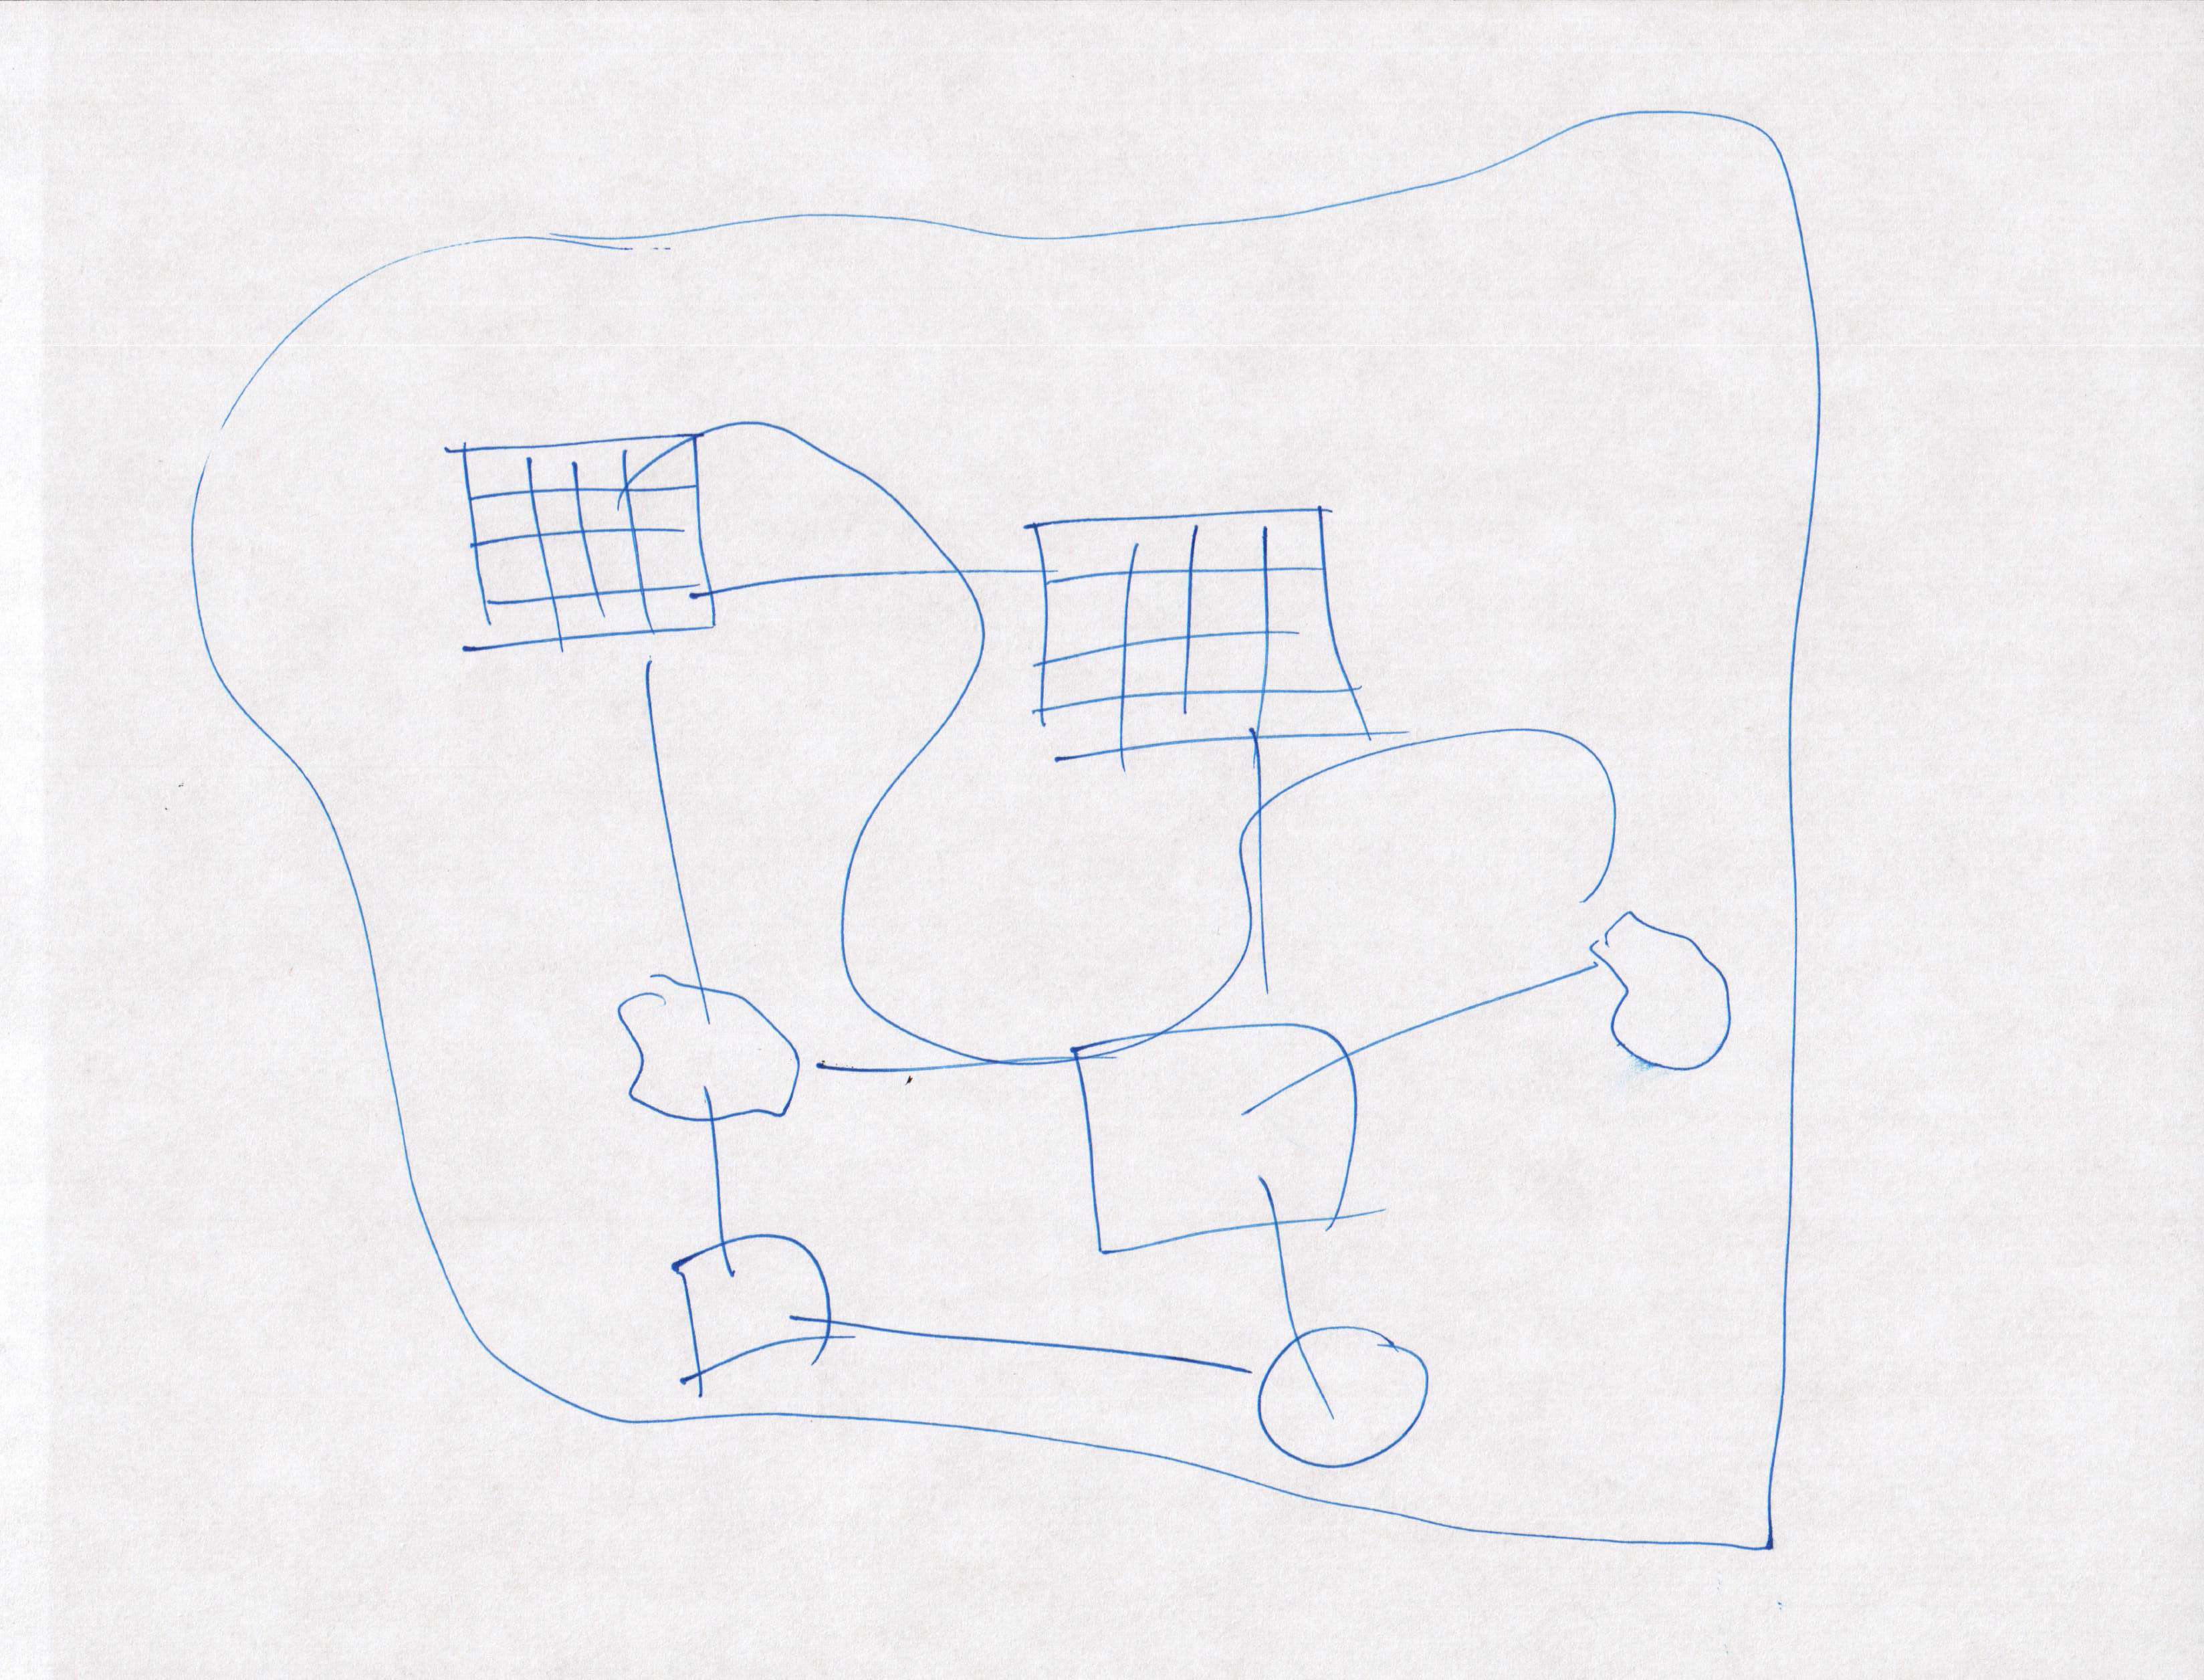
\includegraphics[width=3.45in]{CodeOwnership.jpg}
\caption{\quotes{Draw how you feel about the code}}
\label{Programmer1}
\end{figure}



The team wants to feel \quotes{pride in improving code quality}.  It feels good to be improving the code design and readability. If the team starts neglecting these concerns, it can engender a sense of disgust and an apathy for the code can spread throughout out the team.

\subsubsection{Increasing Product Apathy}
Product apathy occurs when a developer loses investment in the features of the product. Pivotal's balanced team approach is founded on collaboration. When product managers, or other stakeholders, ignore feedback from the developers, the developers can begin to feel less ownership in the product, and in turn be less motivated to work on the project.

When picking up a story, it is the developer's responsibility to verify that the story contains clear acceptance criteria. If it does not, the developer must have a conversation with the product manager to determine what must be done. One developer recalled, \quotes{In this case, I don't feel like spending the extra energy to go and say, `Hey, are you sure? Is this what you want?'} 

Given the technical complexity of a product, sometimes the next story on the backlog can be blocked. Instead of proactively working with product, one developer adopted the attitude: \quotes{Well, this [story] is blocked and it's somebody else's problem.} 

Product apathy can result in a poorly crafted product that does not meet the customer's needs.


\subsubsection{Increasing Team Apathy}
Team Apathy manifests when developers do not feel that they are a part of the team. It is hard to feel collective ownership of the code base when one feels excluded from the collective.

Behaviors we observed that can distance an engineer from the team include: interrupting the engineer during discussions, using poor listening skills so that the developer feels unheard, or talking beyond the engineer's level of technical expertise. 

Poor onboarding of developers also contributes to developers feeling isolated. On one project, there was a time crunch and the team was feeling the pressure to deliver stories. When the team added developers, the team had a \quotes{sink or swim} attitude. For example, the person was left alone with no clear instructions for the first hours on the project. If someone does not feel part of the team, how can they feel ownership of the code base? Making a new team member feel welcomed is important.

On one team, during discussions the team talked about code but never looked at source code. 
For a programmer who learns best visually, it was difficult to follow the discussions. Parts of the code that had not seen recently were difficult for the programmer to visualize; when the team discussed two variants of coding practices without showing concrete examples of the issue, the programmer could not contribute. When the programmer raised this issue to the team, and the team continued with the status quo, the programmer felt marginalized by the team.

%As another developer expressed, \quotes{Not listening to each other can create apathy.}

When developers begins to feel that the team does not care about them, they can begin to care less about the success of the project and the quality of the code base. 

\subsubsection{Decreasing Quality}
A product suffering from quality issues threatens an individual's sense of ownership. First, an engineer may not want to be identified with that product, either internally or externally, to the company. Second, developers need a balance of working on features and fixing bugs each week. Working only on bugs for weeks will affect their sense of ownership.    
 
\subsubsection{Breakdowns in Pair Programming}
When the pairing experience breaks down, one person drives the code development while their partner passively watches. When one person is writing all the code, individual code ownership replaces collective code ownership.  

Reflecting about one particular situation where their pair took over and ignored their input, a developer said, \quotes{I did not understand what was really going on. I wouldn't be able to deeply explain [what we had done]. I wouldn't be able to maintain it. I didn't really write it, so I feel very little ownership of it.} We call this \quotes{Performance Pair Programming}: one developer plows through a story and stops listening to their pair. 

Ideally, Pair Programming is a collaborative experience where both individuals can not tell who wrote which portions of the code. 

In conclusion, we identified several ways in which a team may decrease its sense of collective code ownership: increasing team size, increasing code apathy, increasing product apathy, increasing team apathy, decreasing quality, and breakdowns in pair programming.
\section{Transitioning to Collective Code Ownership}
\label{Transitioning}
Some individuals derive their sense of value, worth, and identity from what they produce. Shifting from individual code ownership to collective code ownership, asks people to shift how they value and perceive themselves, and thus the transition should not be taken lightly.

A recent hire to Pivotal described his initial experience as, \quotes{seeing my work slowly removed from app.} When reflecting on the daily rotation, this developer recalled occasions of wanting to hang onto the work.  In time, his attitude of, \quotes{I want to see it through,} evolved into, \quotes{Someone else is going to take over and they're going to do fine. I can move onto something else and that's okay.} 

The developer learned the rhythm of story rotation and learned to trust in his team: the rest of the team will do a good job. Developers rolling off a story in flight can look in anticipation to see what the next pair produces and see how they solved the problem. 

Eventually, team members recognize the lack of long-term individual authorship, learn to expect their code to be transitory, and thus hold personal contributions more loosely. \quotes{The code that I write today may be in the code base for a little while, but will evolve into something better.}  

Some developers transition easily, and immediately see the benefits of being able to modify any part of the code base. 

One Pivotal engineer uses improv games and collaboration games to help teams to practice letting go of control, trusting the team for the final product, and learning to be pleasantly surprised by what emerges. In this regard, sustainable software development is an ensemble performance. 

The developer transitions from the role of owner to the role of steward or caretaker. In one interview, a Pivot was struggling to describe their relationship with the code on a very challenging project and settled in on the caretaker metaphor : \quotes{Sometimes I kind of feel like a janitor to [the code base].  Maybe caretaker would be better.  Yeah, probably caretaker. I feel like \ldots a janitor just cleans up messes, but a caretaker makes things better.}

%tmp comment to get paper into 6 pages
%Our ability to control something influences our sense of ownership, and ownership influences our sense of identity. 

For someone transitioning to collective code ownership with strong individual ownership tendencies, we recommend starting that person on a four person team. This will allow the person to see the benefits of shared code ownership while slowly practicing the release of individual ownership. On a four person team, each daily rotation creates pairs with full knowledge of what happened yesterday.  

When a team achieves a sense of collective ownership, the magic happens: \quotes{People are a lot more flexible all across the board with changing things or accepting feedback or collaborating,} and, \quotes{We want the best possible product that's best for users \ldots we just want the best thing out there.} Then the team can say, \quotes{Hey, this is our code!}

\section{Theory Evaluation}
\label{TheoryEvaluation}

In assessing a Grounded Theory research study, Charmaz identifies four criteria for evaluating a grounded theory study: credibility, (\quotes{is there sufficient data}), originality, (\quotes{do the categories offer new insights}), resonance (\quotes{does the theory make sense to participants}), usefulness (\quotes{does the theory offer useful interpretations}) \cite{StolGTinSE}. 

\begin{itemize}
\item 
\textbf{credibility:}  The number of open ended interviews and the field notes from participant observation serve as a rich data set for the analysis. 
%The developer staffing for the project serves as a compelling illustration of the theory in practice

\item
\textbf{originality:} Extreme Programming discusses Pair Programming and Continuous Refactoring. This paper adds the overlapping pair rotation practice as a means of removing knowledge silos. This paper also broadens the definition of collective code ownership by acknowledging that a team may loose its sense of ownership when certain activities occur.

\item
\textbf{resonance:} When shown to participants, they understand why collective code ownership can be eroded and how to work against that erosion.

\item
\textbf{usefulness:} 
When shown to participants, they immediately understand the theory and better understand why Pivotal follows certain practices. 
\end{itemize}

\section{Threats to Validity}

\subsection{External Validity}

\textbf{Generalizability across situations:} a grounded theory limitation is that the theory emerges from a particular context and may not be applicable to other situations. This work analyzed software projects at the Silicon Valley office of Pivotal following Extreme Programming. The results might not be applicable to other teams in industry wanting collective code ownership or  following Extreme Programming. Replicating the results with other teams would mitigate this threat. 

\subsection{Internal Validity}
\textbf{Researcher bias:} a risk of the participant-observer technique is that the researcher may lose perspective and become biased by being a member of the team. An outside observer might see something the researcher missed. We mitigated this risk by recording interviews and with a colleague reviewing the coding process. 

\textbf{Prior knowledge bias:} with grounded theory prior knowledge can aid the researcher in looking at interesting research questions or create difficulties in blinding the researcher about possible explanations. \cite{GlaserIssues}. We mitigated this risk with a colleague reviewing the coding process. 

\section{Future Research}
Developers, designers, and product managers all have different goals in their roles. In future work, we plan to examine how collective ownership is driven by different factors for designers, developers, and product managers.

Some programmers naturally adapt to collective code ownership, while others struggle with the transition. In future research we will follow new Pivotal engineers and examine their journey in transitioning from individual to collective code ownership. This may uncover specific practices that Pivotal or the development team could employ ease the transition. 

%Further research is necessary to determine the optimal team size for collective code ownership. Early indications suggest that a four person team is a optimal for introducing collective code ownership. With a four person team, each pair  is working on half of the new feature development. When they rotate the next day, each developer will be paired with a developer from the other pair. This way, no individual developer is ever left feeling isolated or in a code silo, since their pair can bring them up to speed quickly on all changes. This helps ensure they continue to feel part of the team and fights (various types of) apathy.

\section{Conclusions}
For a team to achieve a high sense of collective code ownership, it must actively remove knowledge silos. The practices of Pair Programming, Overlapping Pair Rotation, and Continuous Refactoring enables a team to share context and not have silo ownership. 

Many factors can weaken a team's sense of collective code ownership. Teams can proactively engage to either mitigate against these risks or overcome issues as they arise based on their style and team dynamics. 

Transitioning to collective code ownership is not easy. In time, developers learn to loosely hold personal contributions and recognize the lack of long term individual authorship. Then they can switch from \quotes{I made this} to \quotes{we made this.}

% The primary benefit to the employer is business agility. The engineering team continues to deliver software week after week, month after month, and survive cataclysmic events. Things do not fall apart when the superstar developer leaves. People can go on vacation whenever they need to because features or components are not critically tied to a particular individual. The team leverages the whole team's talents. This removes bottlenecks of, \textif{Only Pat can work on these features.} Critical feature work can be parallelized since anyone can work on the feature, as opposed to an individual code owner. 

% The primary benefit to the engineering team is the ability to work on every story, to understand the entire system, teaching opportunities to share one's expertise and to deeper learn subtle parts of the technologies. 

% The primary cost is a shift from individual code ownership to collective code ownership. For some engineers, their sense of value and self-worth is derived from direct code ownership, and thus transitions to Sustainable Software Development should not be taken lightly. Sustainable Software Development works well with collaborative individuals and may not be suited for people who like to work on their own. Sustainable Software Development works when team members have the maturity to loosely hold temporary personal contributions understanding that the team may enhance any aspect of the product.

% Sustainable Software Development is suited for companies that must routinely deliver value to their customers or stakeholders. Some companies are better positioned to withstand a quarter where nothing happens (from an external perspective) or  \quotes{the forgotten two years of management waste} as described by one manager in this study. Hopefully, competitors have not caught up or surpassed the organization during the lost time. Both Pivotal Labs as a consulting practice and the growth of Pivotal's Cloud Foundry towards market dominance, depend on the continual development of features. Neither can afford to falter and both implement Sustainable Software Development.

% Sustainable Software Development is that software development continues at a regular pace regardless of who is on the team, or rather regardless of changes in team composition.


